%!TEX root = ../thesis.tex

\renewcommand{\thefigure}{A\arabic{figure}}
\setcounter{figure}{0}

% ---
% #1
% ---
\thispagestyle{empty}
\section*{APPENDIX 1. Application demonstration}

\vfill

\begin{figure}[ht]
  \centering
  \captionsetup{justification=centering,margin=0.2cm}
  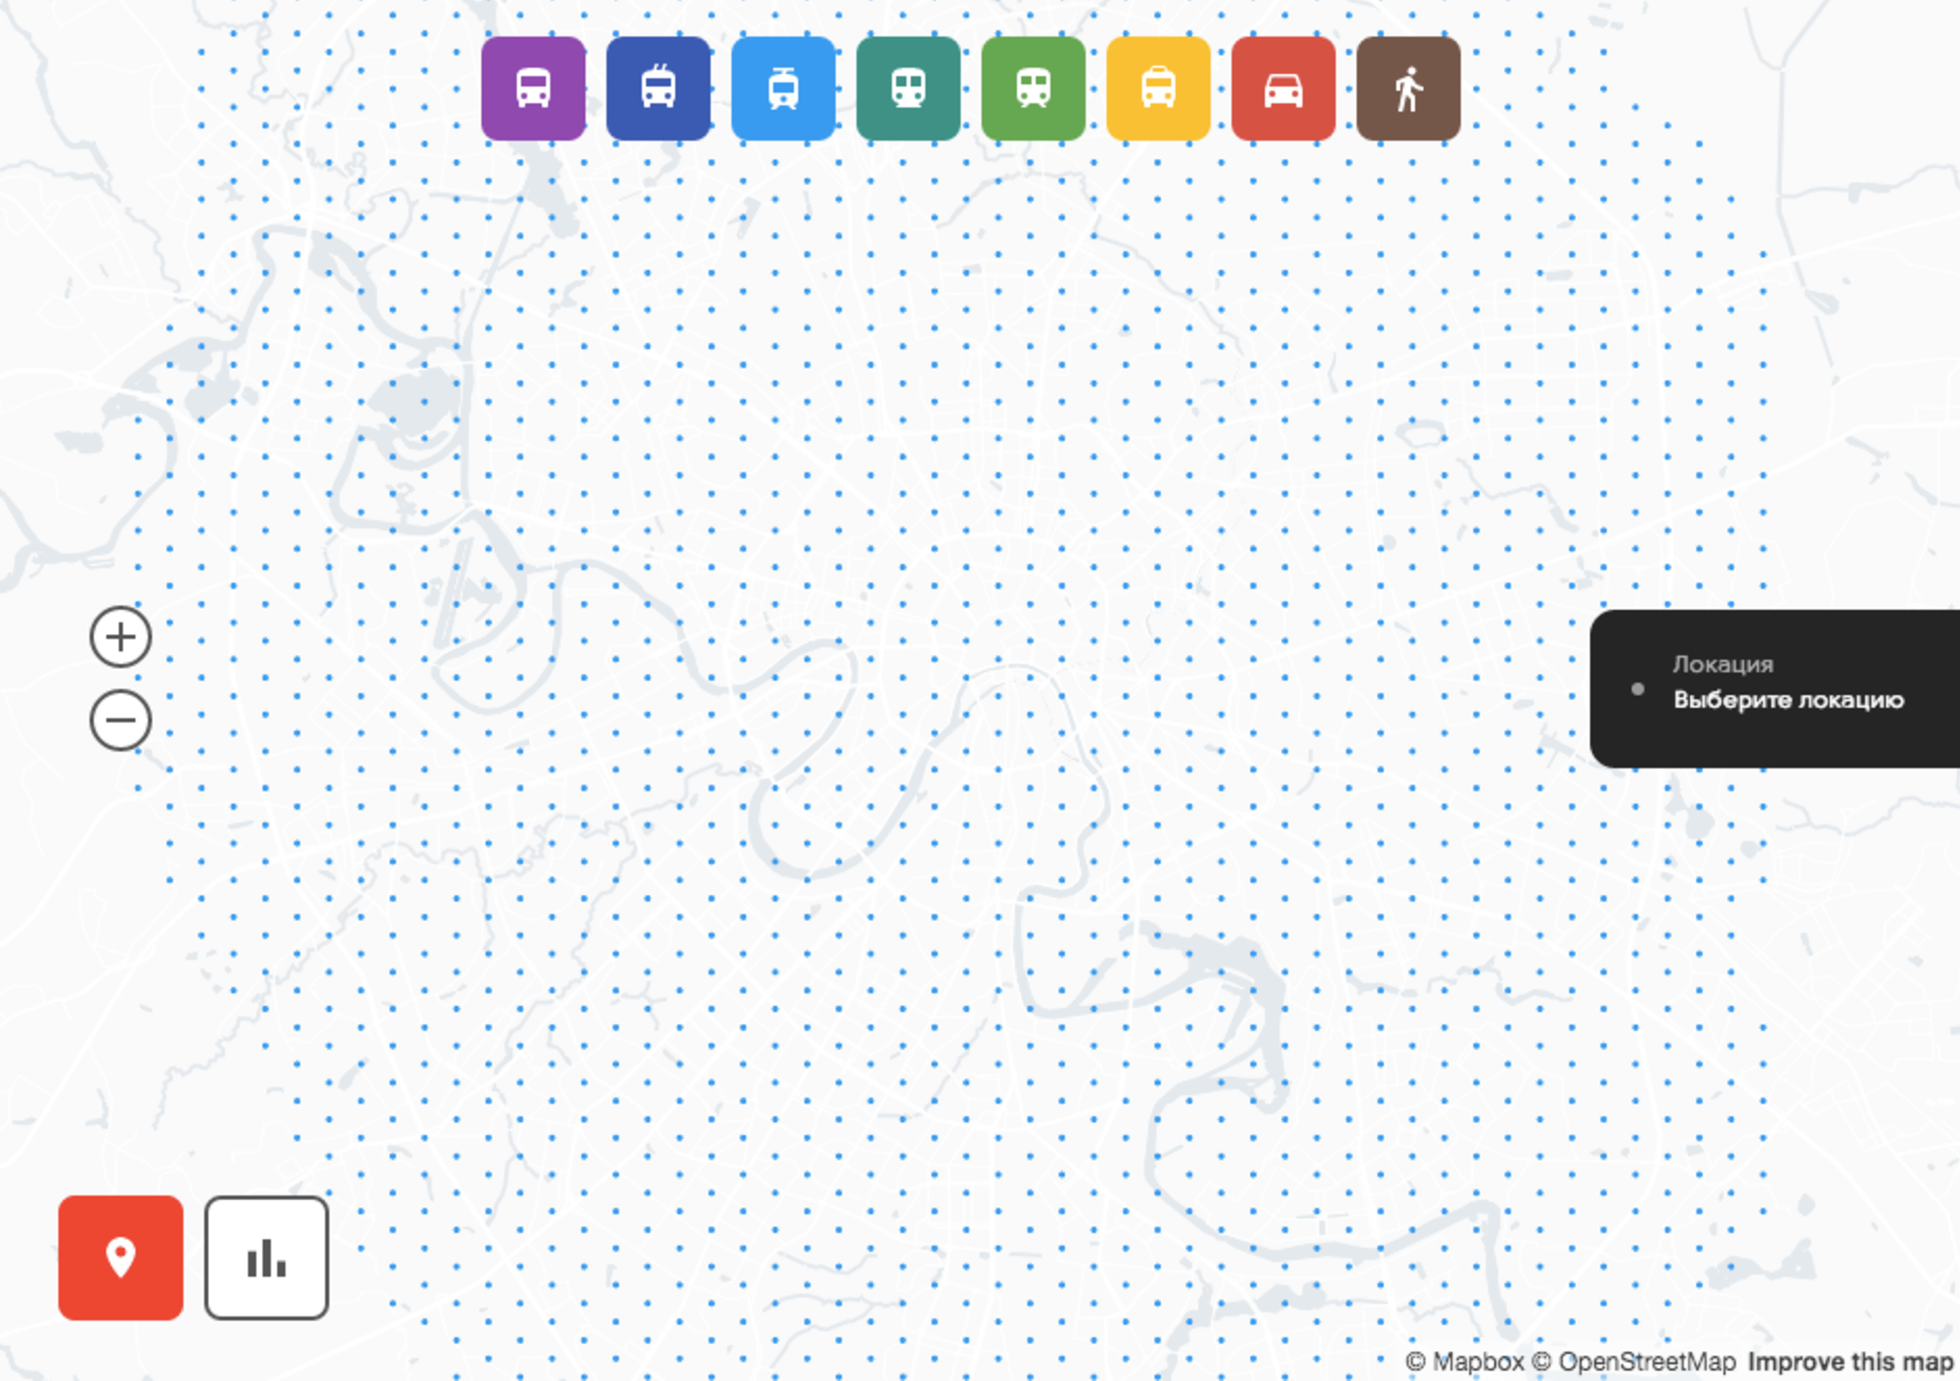
\includegraphics[width=1\textwidth]{start-state.pdf}
  \caption{Inital application state where user can select particular location for analysis.}
  \label{pic:startstate}
\end{figure}

\vfill
\begin{flushright}
  (continues)
\end{flushright}

% ---
% #2
% ---
\thispagestyle{empty}
\section*{APPENDIX 1. (continues)}

\vfill

\begin{figure}[ht]
  \centering
  \captionsetup{justification=centering,margin=0.2cm}
  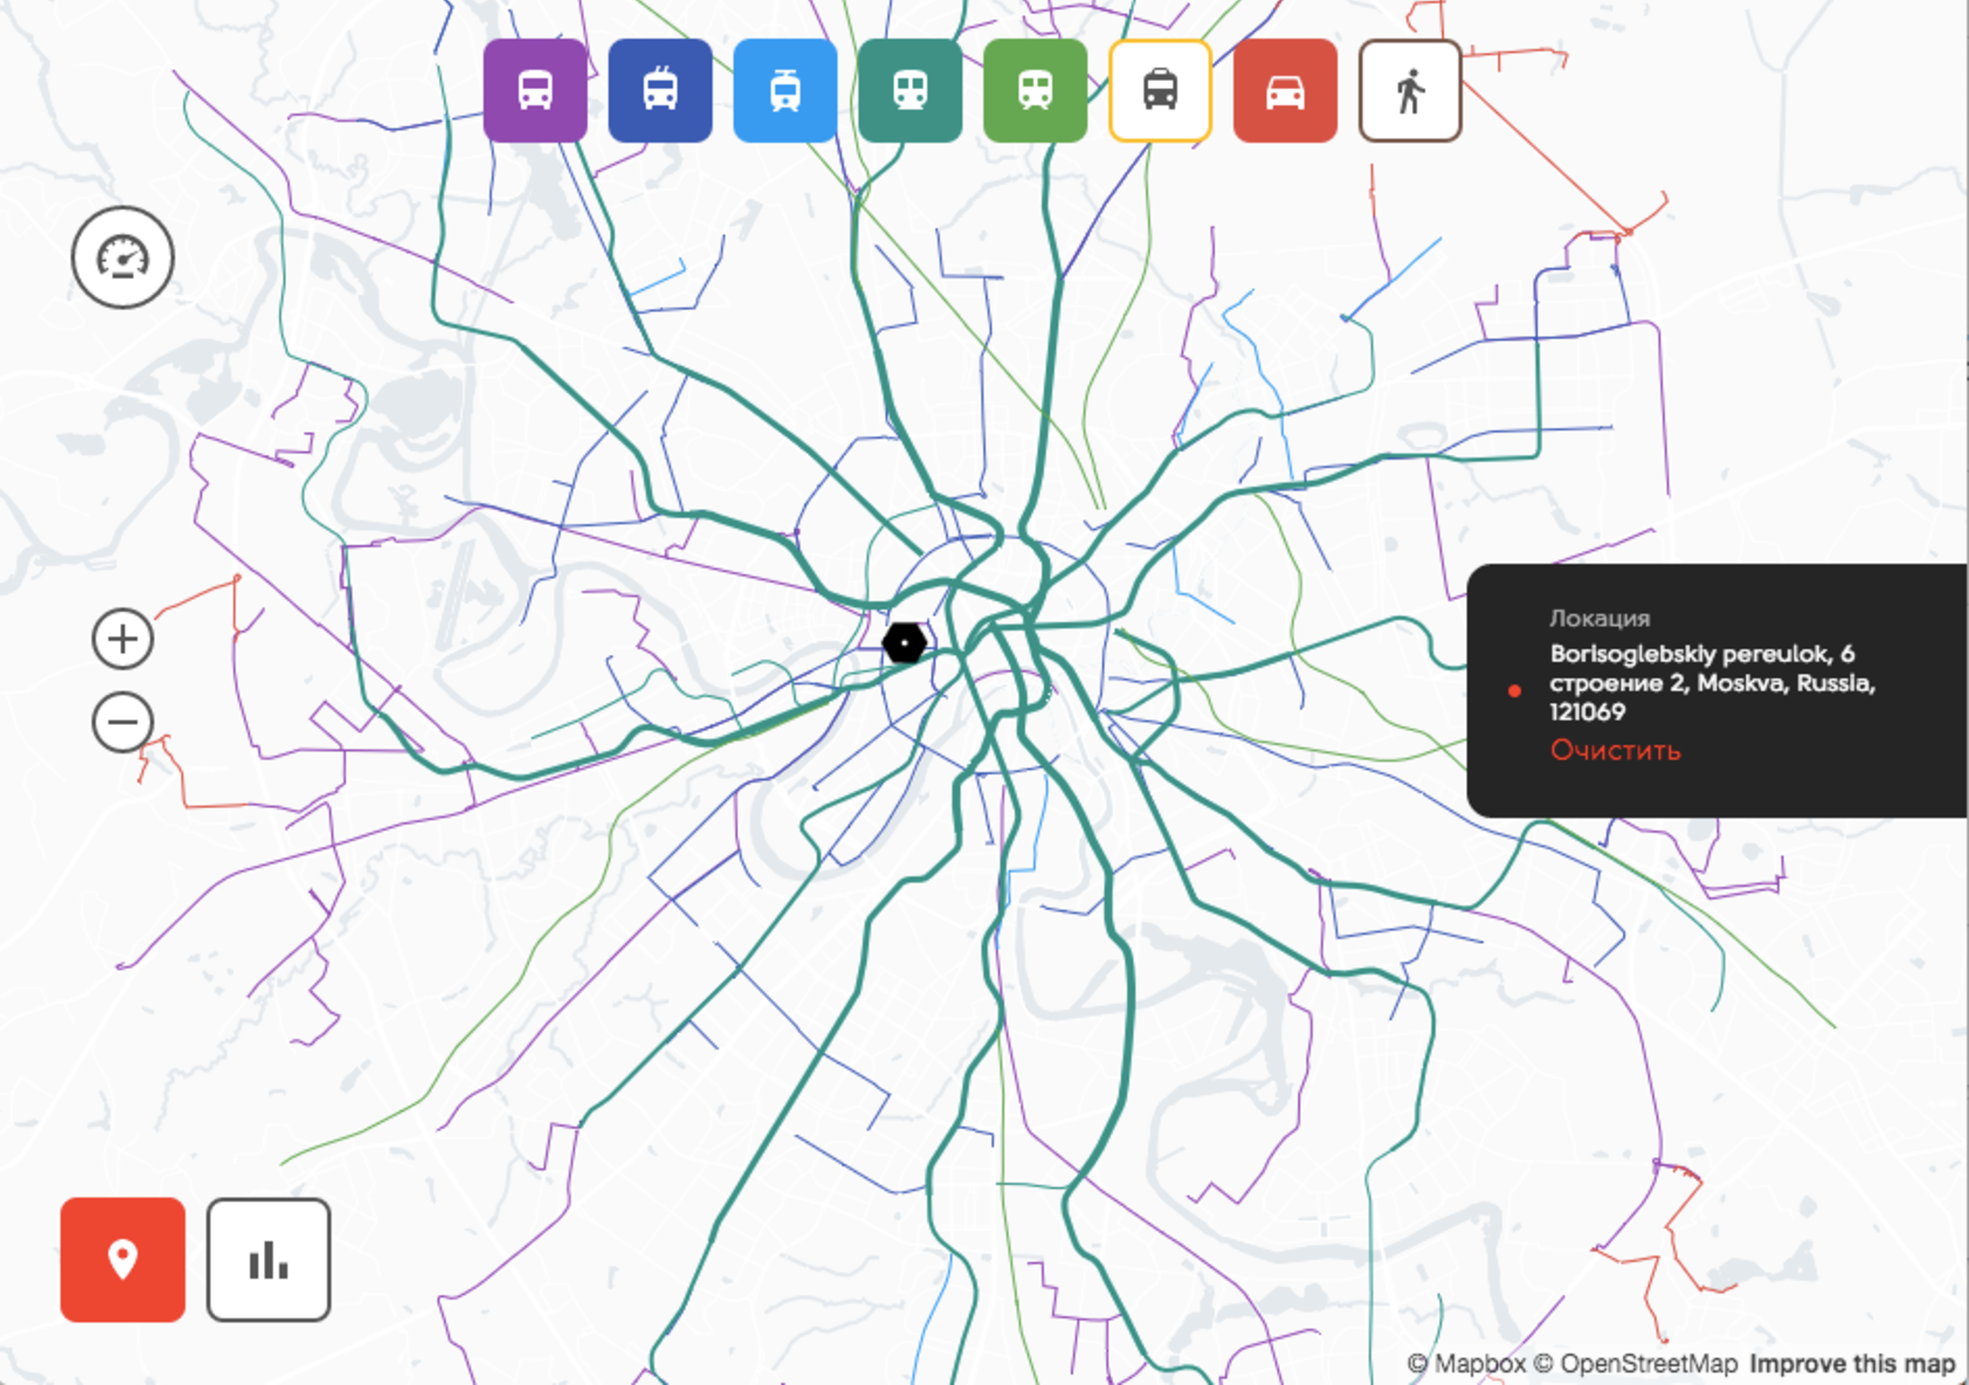
\includegraphics[width=1\textwidth]{point-state.pdf}
  \caption{The state when user selected particular location switched off ``share taxi'' and
  ``walking'' transport types.}
  \label{pic:pointstate}
\end{figure}

\vfill
\begin{flushright}
  (continues)
\end{flushright}

% ---
% #3
% ---
\thispagestyle{empty}
\section*{APPENDIX 1. (continues)}

\vfill

\begin{figure}[ht]
  \centering
  \captionsetup{justification=centering,margin=0.2cm}
  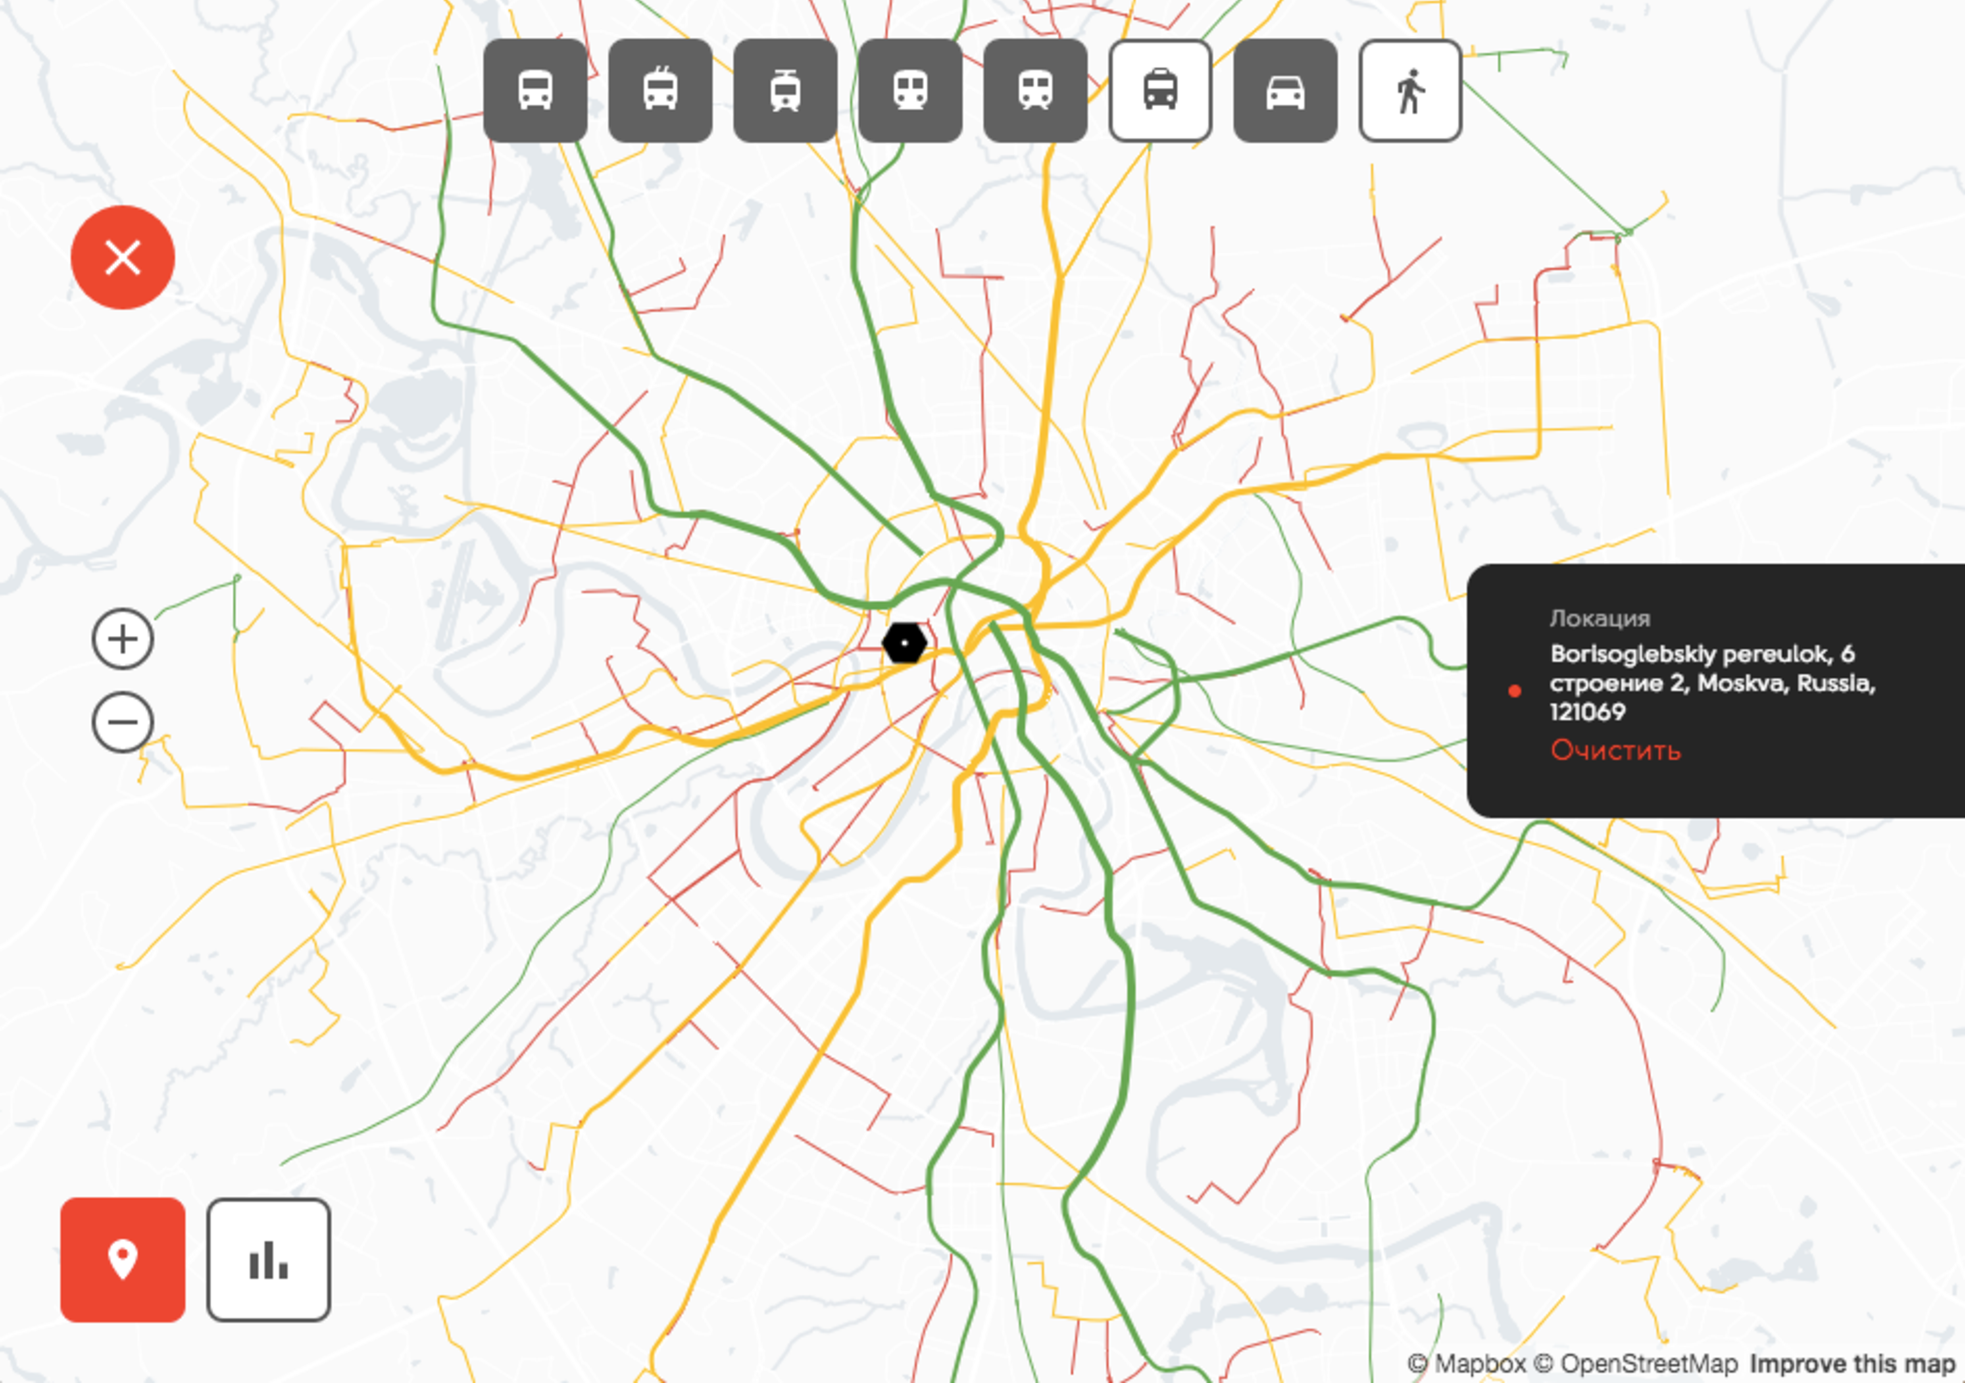
\includegraphics[width=1\textwidth]{speed-state.pdf}
  \caption{User selected location and switched to speed map.}
  \label{pic:speedstate}
\end{figure}

\vfill
\begin{flushright}
  (continues)
\end{flushright}

% ---
% #4
% ---
\thispagestyle{empty}
\section*{APPENDIX 1. (continues)}

\vfill

\begin{figure}[ht]
  \centering
  \captionsetup{justification=centering,margin=0.2cm}
  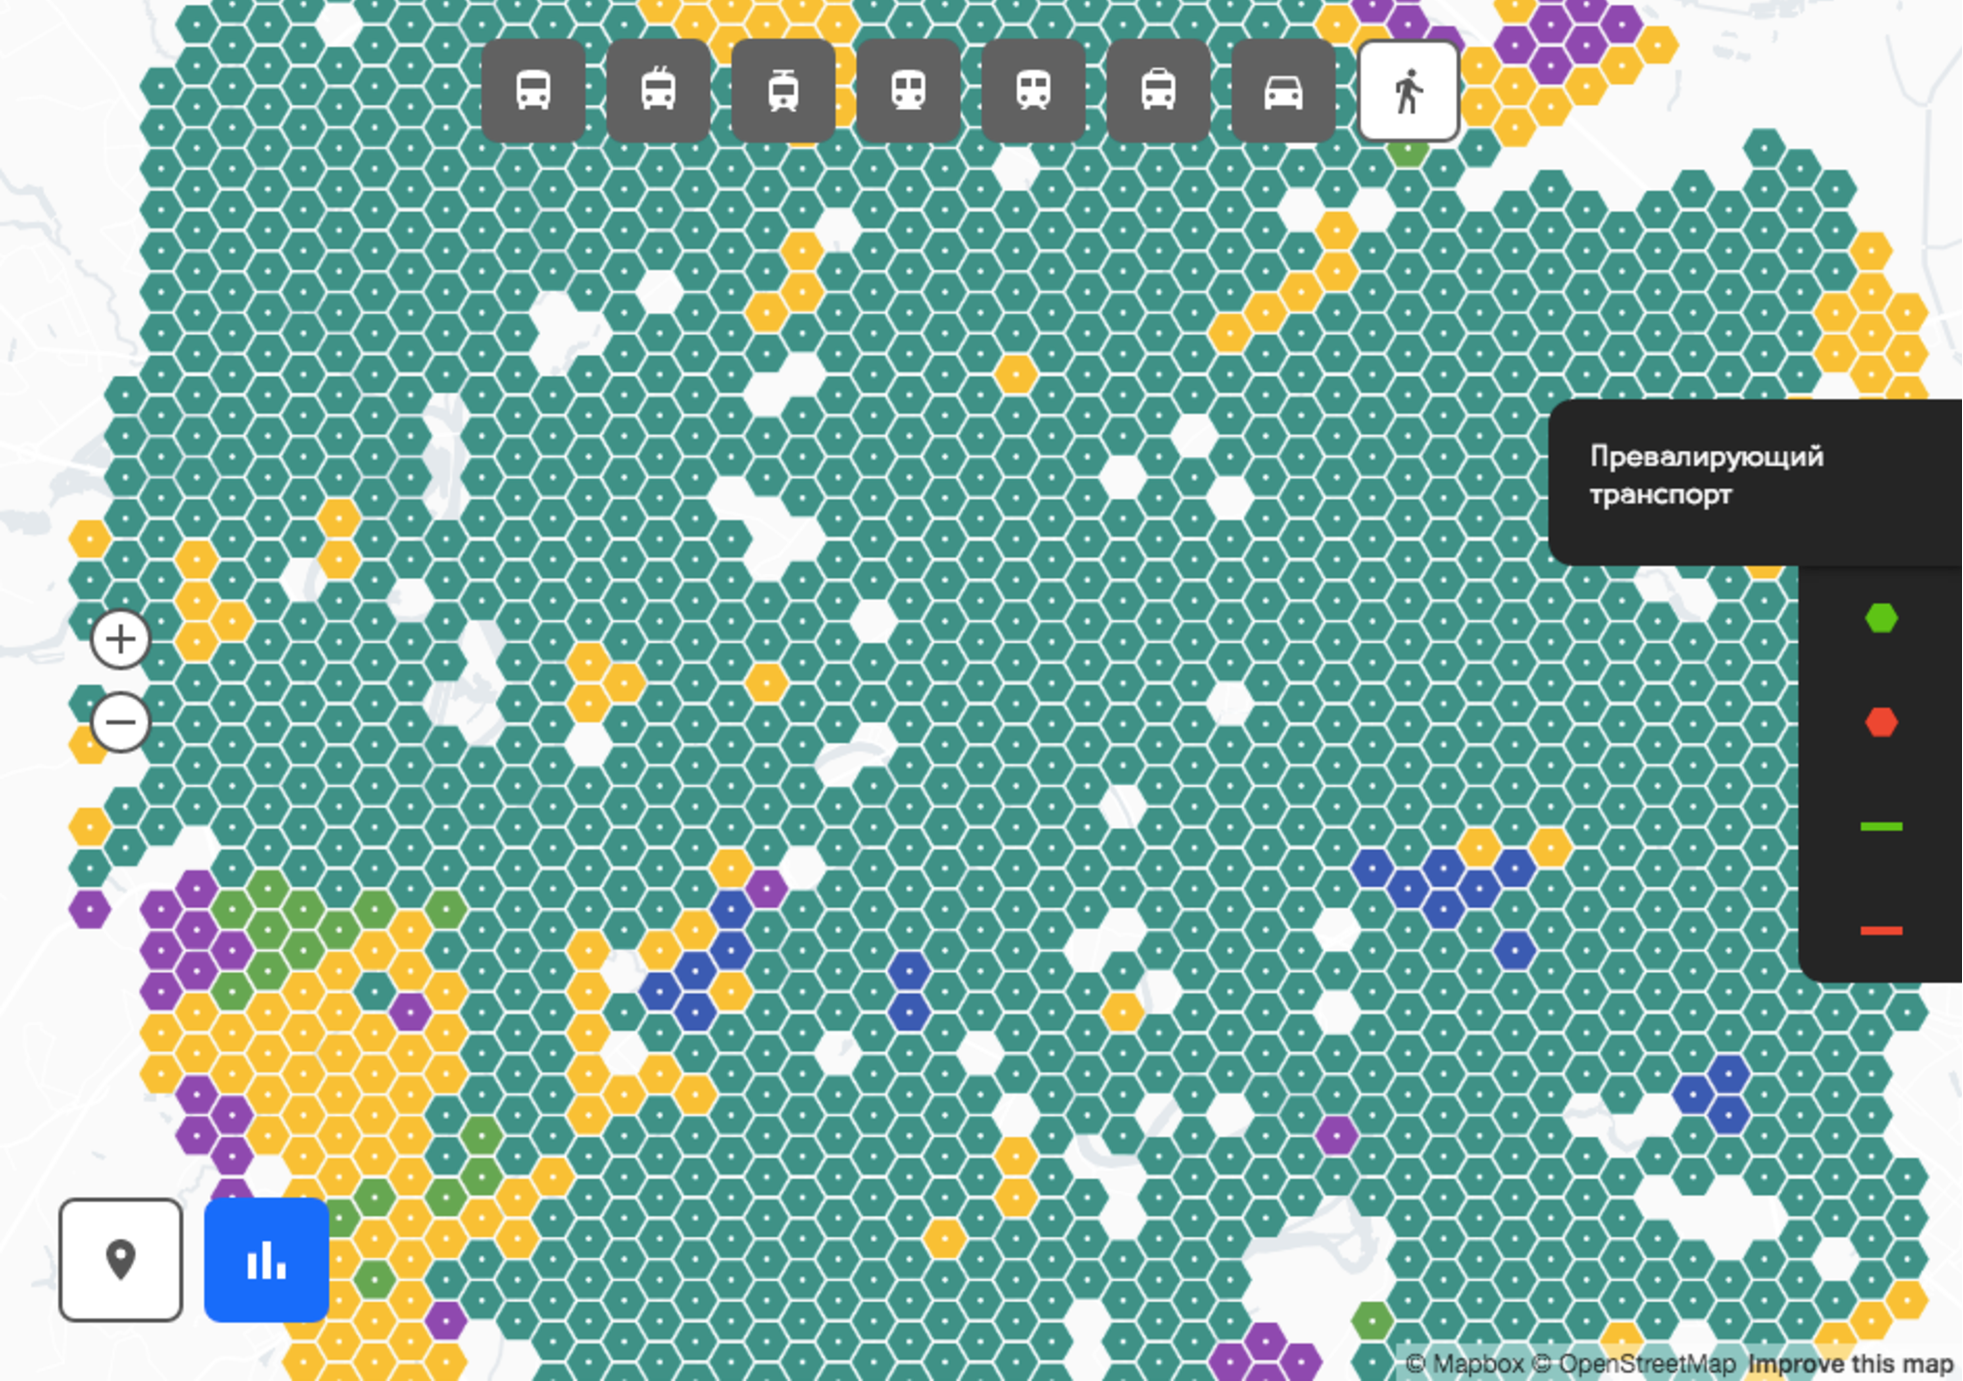
\includegraphics[width=1\textwidth]{transport-state.pdf}
  \caption{Prevailing transport.}
  \label{pic:transportstate}
\end{figure}

\vfill
\begin{flushright}
  (continues)
\end{flushright}

% ---
% #5
% ---
\thispagestyle{empty}
\section*{APPENDIX 1. (continues)}

\vfill

\begin{figure}[ht]
  \centering
  \captionsetup{justification=centering,margin=0.2cm}
  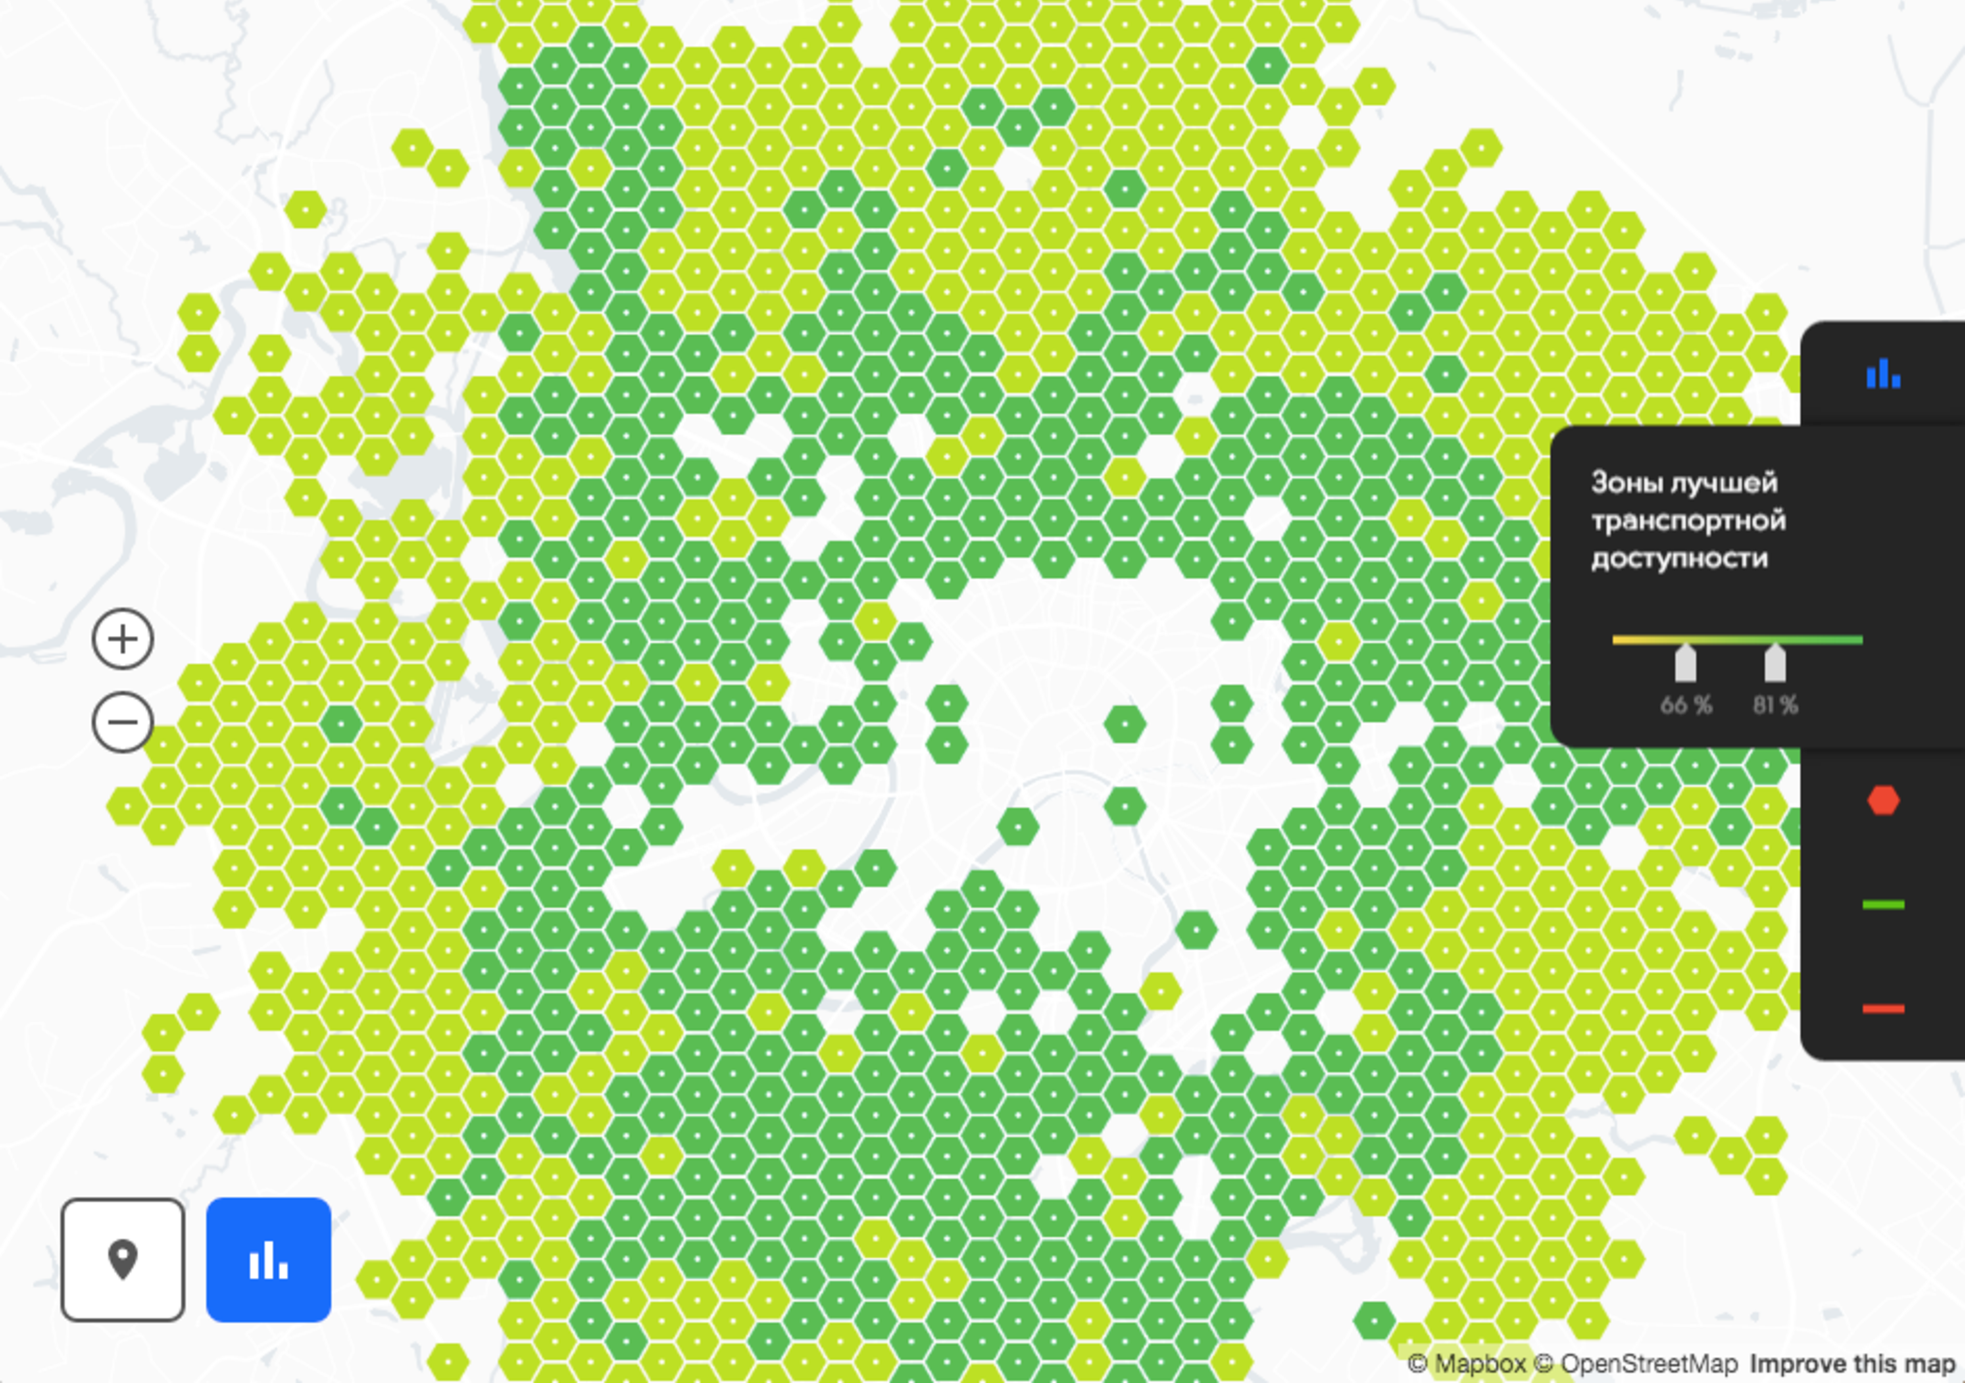
\includegraphics[width=1\textwidth]{mostacc-state.pdf}
  \caption{Most accessible locations with range filter.}
  \label{pic:mostaccstate}
\end{figure}

\vfill
\begin{flushright}
  (continues)
\end{flushright}

% ---
% #6
% ---
\thispagestyle{empty}
\section*{APPENDIX 1. (continues)}

\vfill

\begin{figure}[ht]
  \centering
  \captionsetup{justification=centering,margin=0.2cm}
  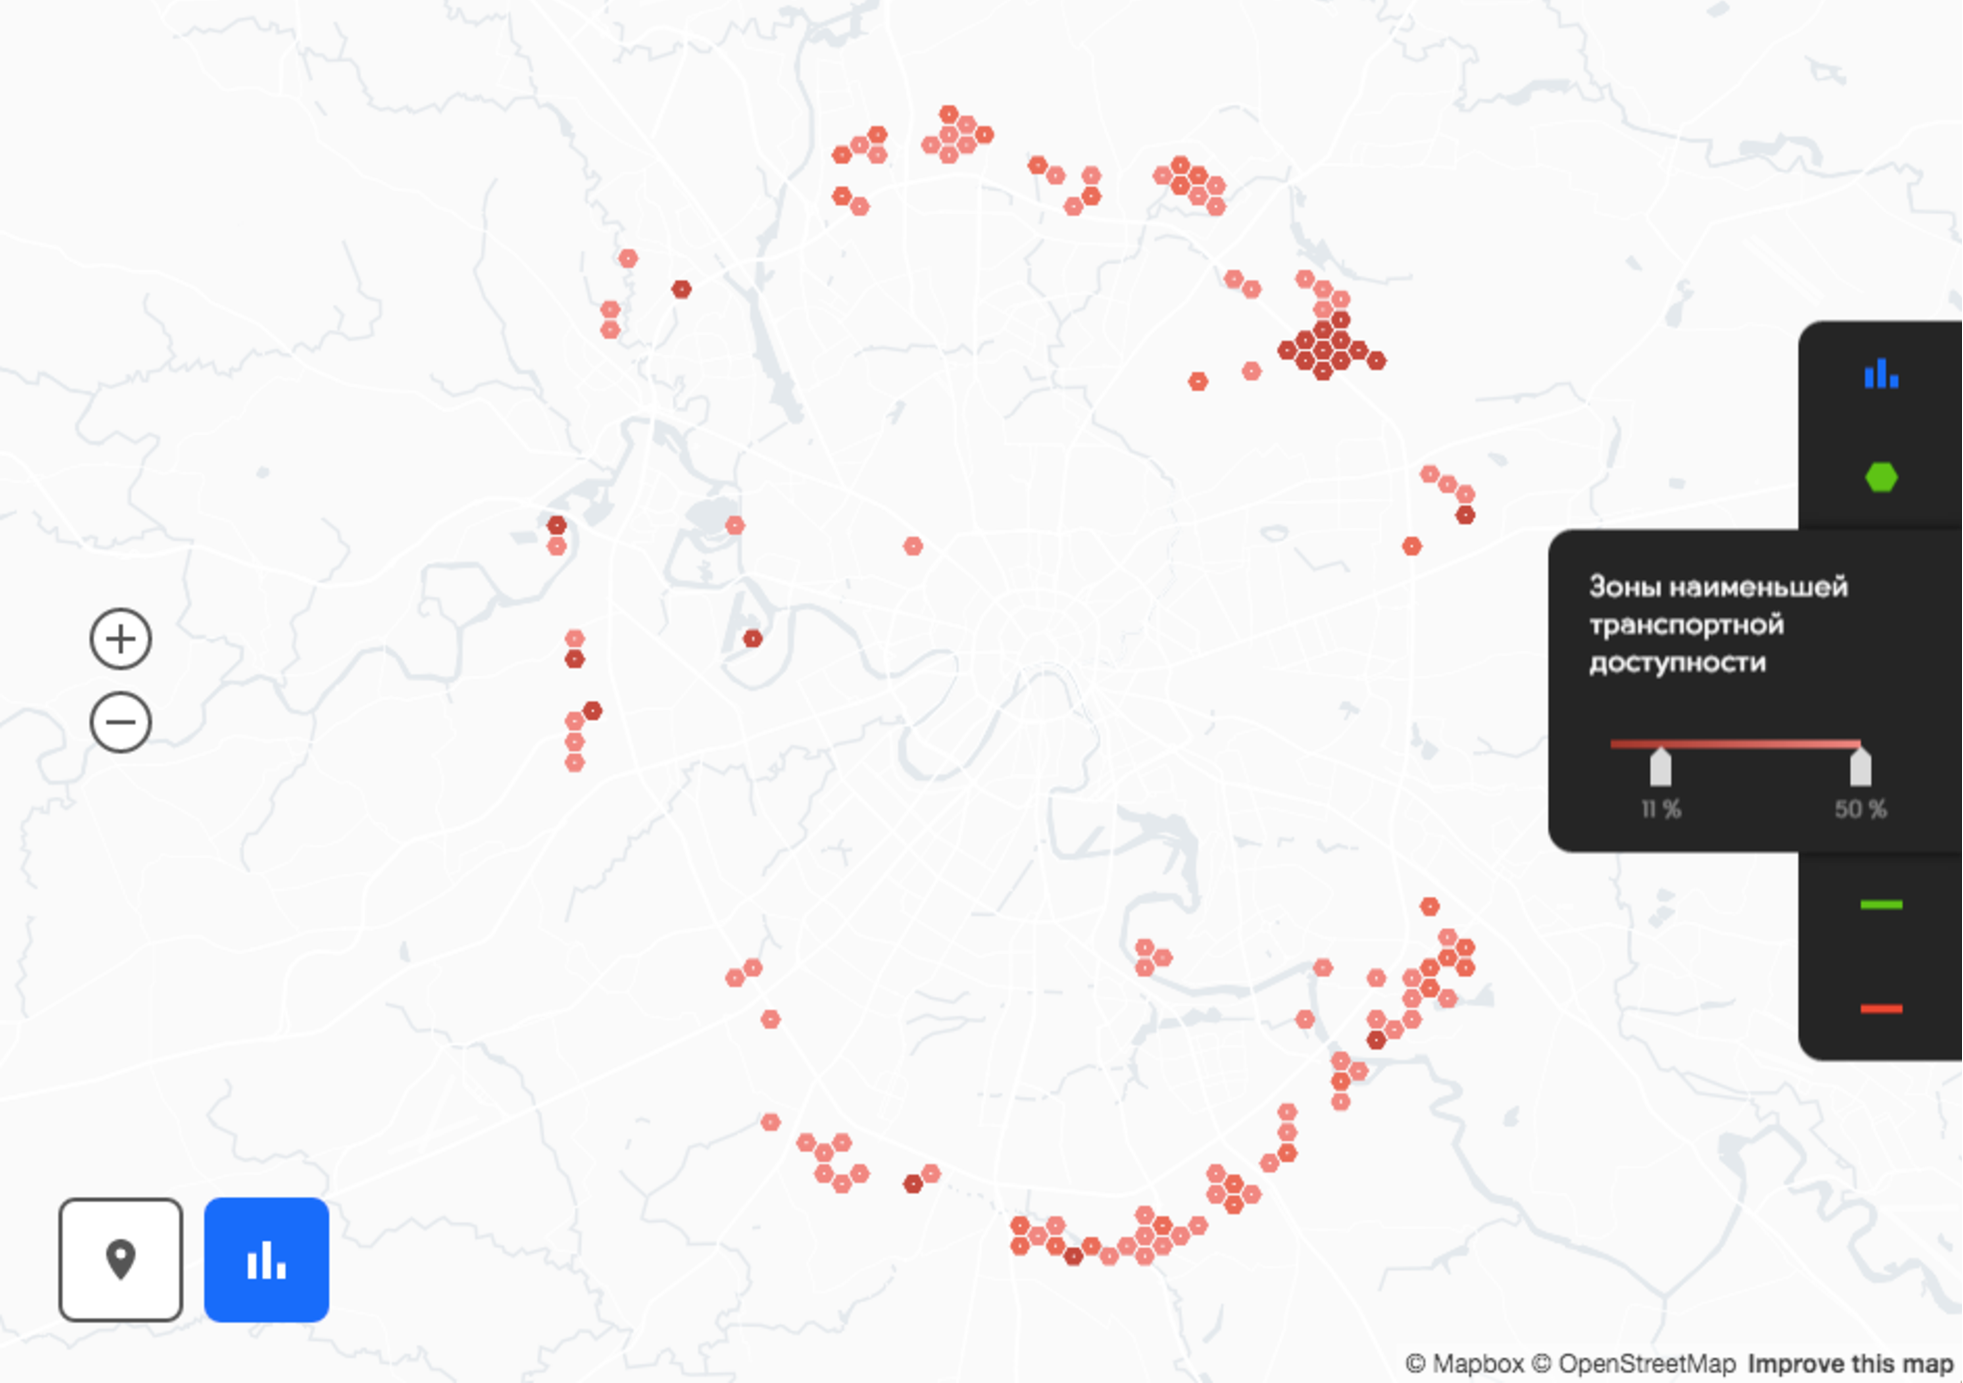
\includegraphics[width=1\textwidth]{leastacc-state.pdf}
  \caption{Least accessible locations with range filter.}
  \label{pic:leastaccstate}
\end{figure}

\vfill
\begin{flushright}
  (continues)
\end{flushright}

% ---
% #7
% ---
\thispagestyle{empty}
\section*{APPENDIX 1. (continues)}

\vfill

\begin{figure}[ht]
  \centering
  \captionsetup{justification=centering,margin=0.2cm}
  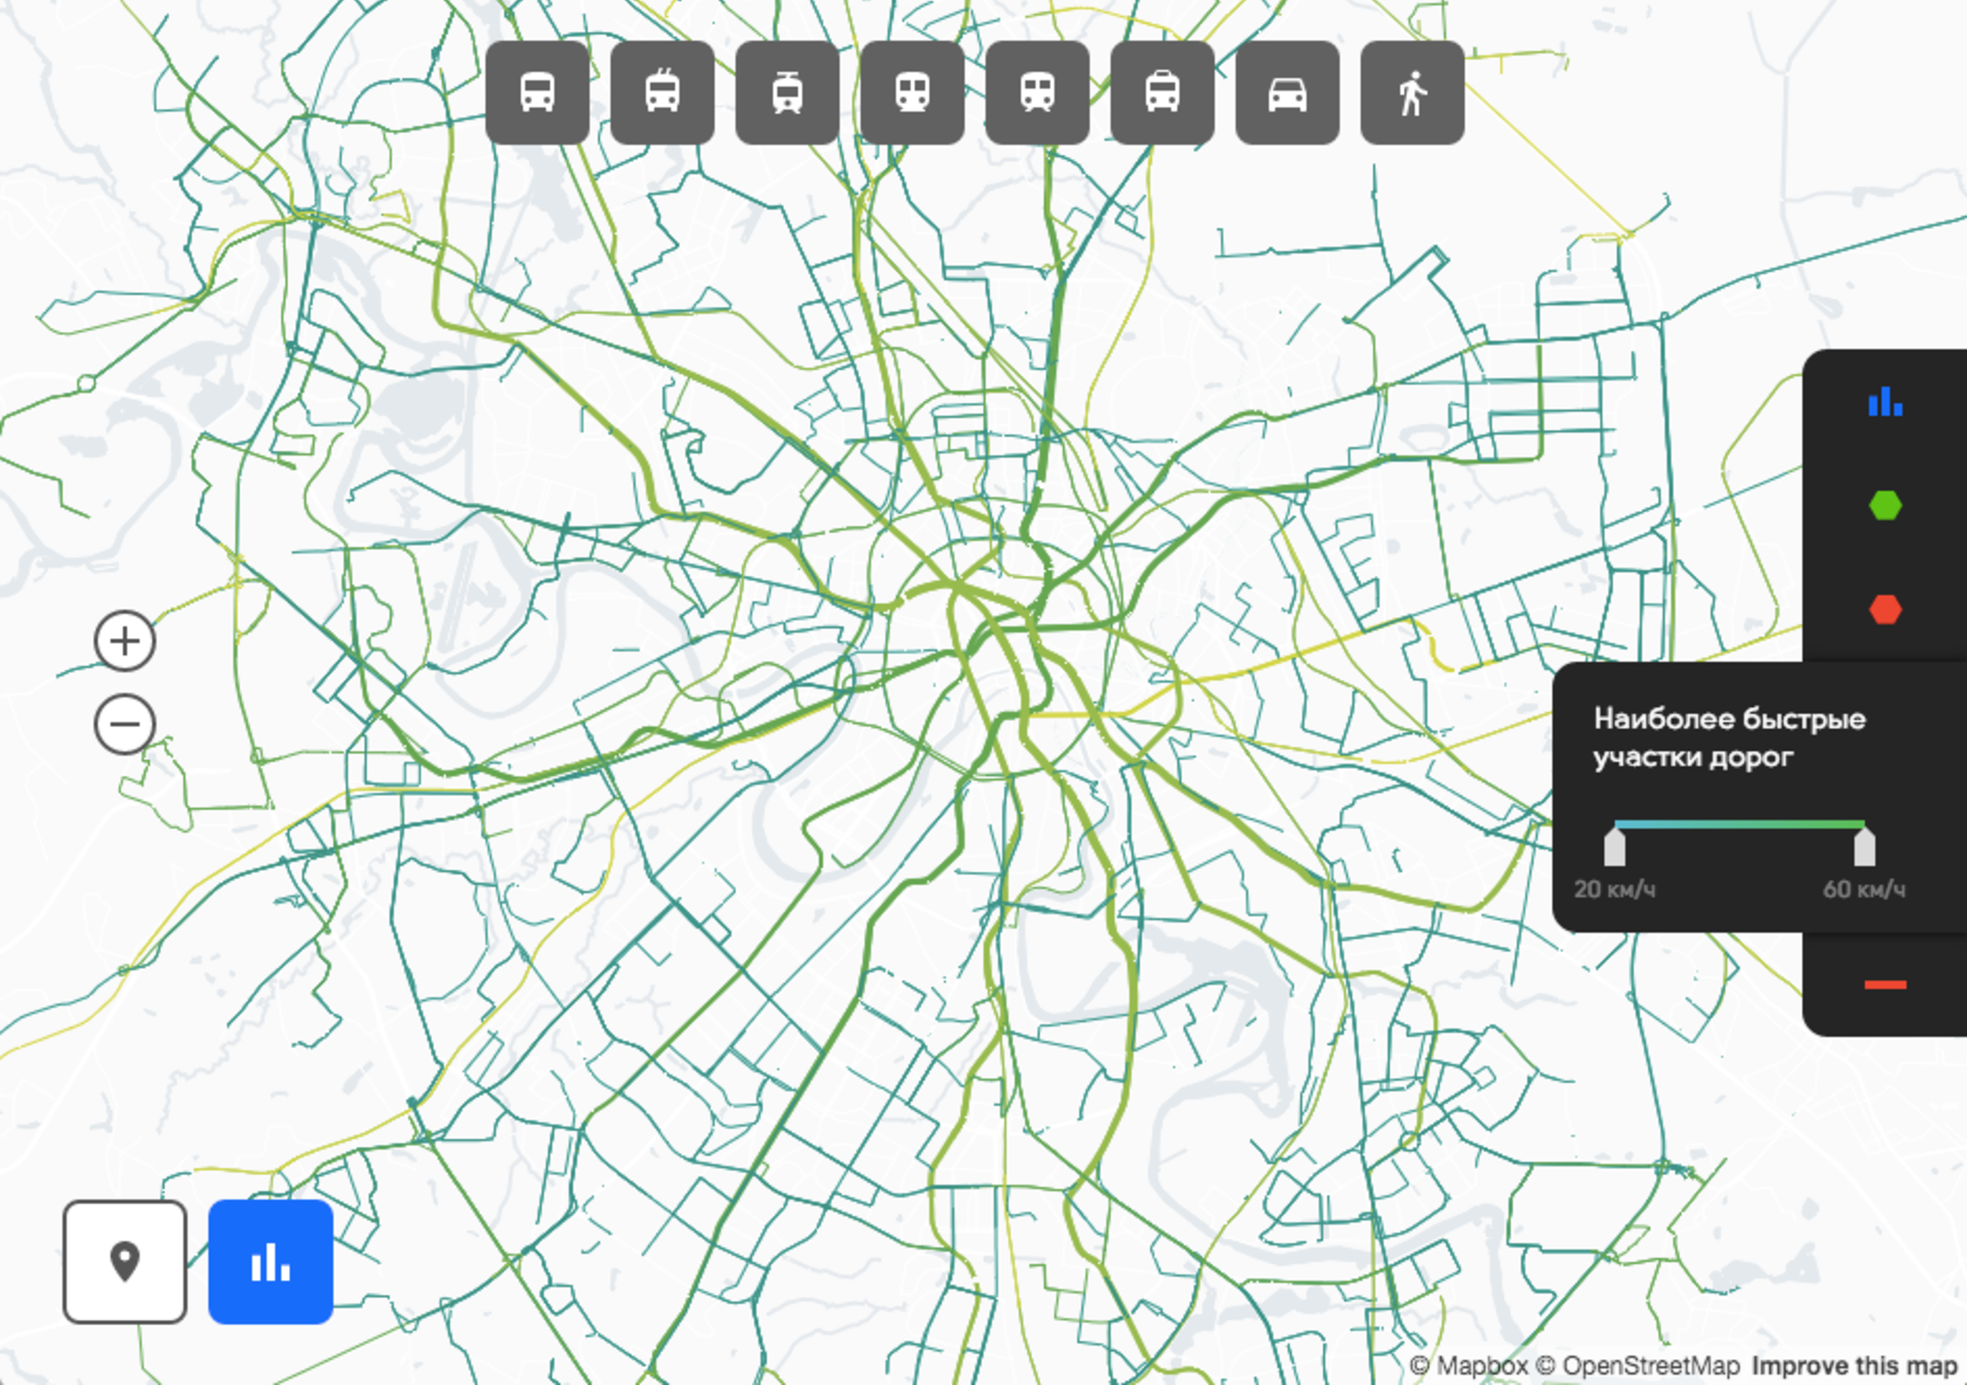
\includegraphics[width=1\textwidth]{fastest-state.pdf}
  \caption{Fastest parts of the routes with filter by speed.}
  \label{pic:fasteststate}
\end{figure}

\vfill
\begin{flushright}
  (continues)
\end{flushright}

% ---
% #7
% ---
\thispagestyle{empty}
\section*{APPENDIX 1. (continues)}

\vfill

\begin{figure}[ht]
  \centering
  \captionsetup{justification=centering,margin=0.2cm}
  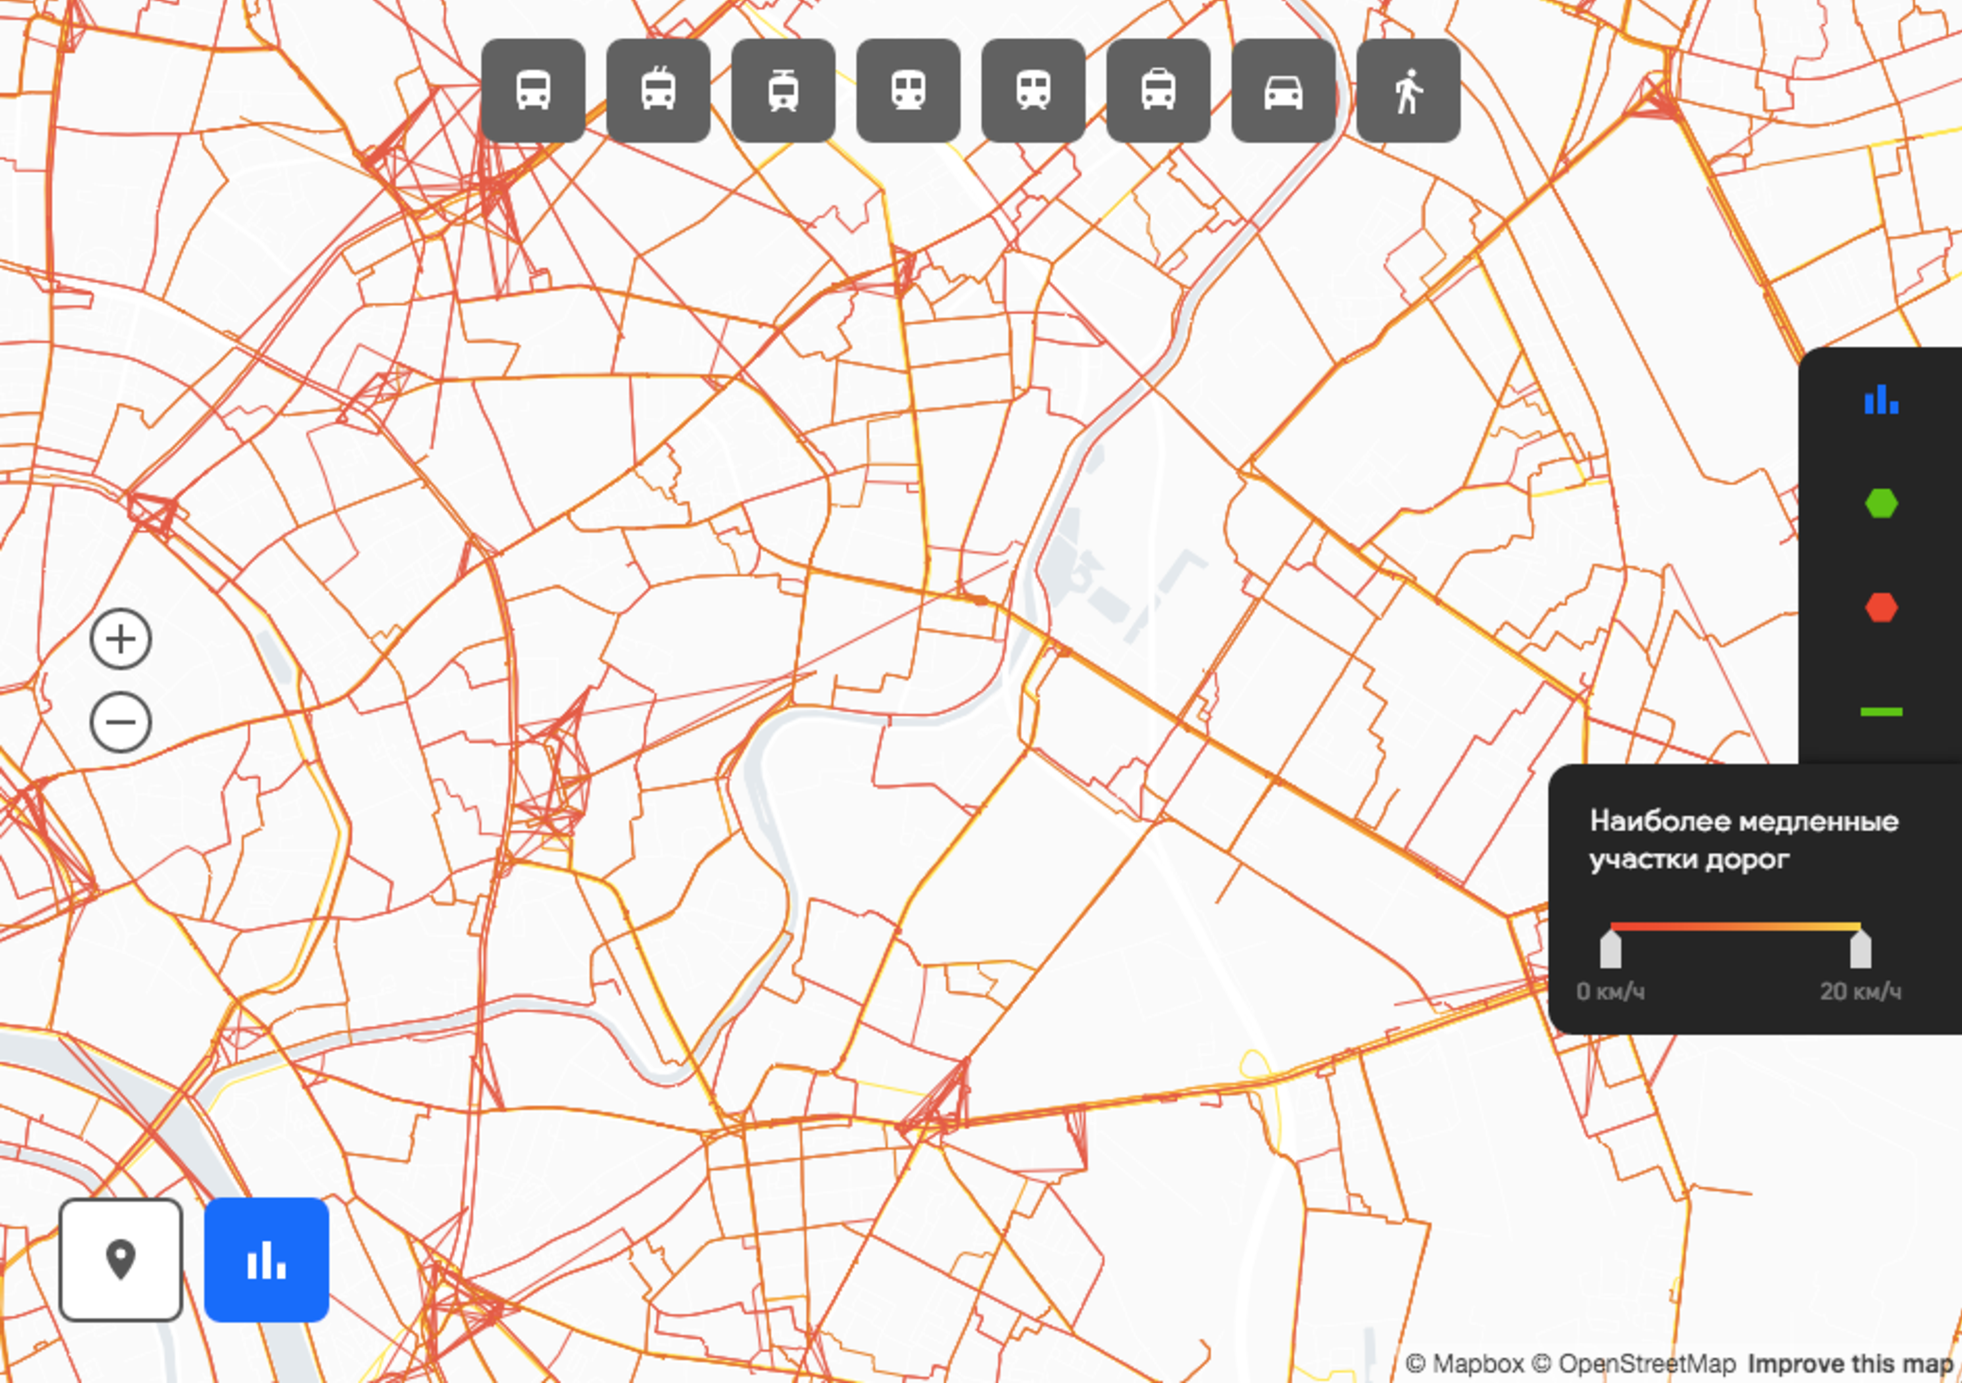
\includegraphics[width=1\textwidth]{slowest-state.pdf}
  \caption{Slowest parts of the routes with filter by speed.}
  \label{pic:sloweststate}
\end{figure}

\vfill

\thispagestyle{empty}